\documentclass[aspectratio=169,11pt]{beamer}
\usepackage[spanish,es-nodecimaldot]{babel}
\usepackage{amsmath,amssymb,graphicx}
\usepackage{lmodern}
\renewcommand{\ttdefault}{lmss}

\definecolor{Noche}{HTML}{12263A}
\definecolor{Petroleo}{HTML}{1B4965}
\definecolor{Turquesa}{HTML}{2A9D8F}
\definecolor{Coral}{HTML}{E76F51}
\definecolor{Hielo}{HTML}{EAF4F4}
\definecolor{Gris}{HTML}{52606D}
\setbeamercolor{normal text}{fg=Noche,bg=white}
\setbeamercolor{structure}{fg=Petroleo}
\setbeamercolor{frametitle}{fg=Noche,bg=white}
\setbeamercolor{block title}{fg=white,bg=Petroleo}
\setbeamercolor{block body}{fg=Noche,bg=Hielo}
\setbeamercolor{alerted text}{fg=Coral}
\setbeamertemplate{navigation symbols}{}
\setbeamertemplate{items}[circle]
\setbeamertemplate{frametitle}{\vspace{0.18cm}\insertframetitle\par\vspace{0.02cm}{\color{Turquesa}\rule{1.35cm}{1.7pt}}}
\setbeamertemplate{footline}{%
\leavevmode\hbox{%
\begin{beamercolorbox}[wd=.88\paperwidth,ht=2.7ex,dp=1.1ex,leftskip=.55cm]{author in head/foot}%
\color{Gris}\scriptsize Ide y Talam\`as (2025) --- IA en la econom\'ia del conocimiento
\end{beamercolorbox}%
\begin{beamercolorbox}[wd=.12\paperwidth,ht=2.7ex,dp=1.1ex,center]{author in head/foot}%
\color{Petroleo}\scriptsize\insertframenumber/\inserttotalframenumber
\end{beamercolorbox}}\vskip0pt}
\setbeamerfont{title}{size=\fontsize{25}{29}\selectfont,series=\bfseries}
\setbeamerfont{frametitle}{size=\Large,series=\bfseries}
\newcommand{\clave}[1]{\textcolor{Petroleo}{\textbf{#1}}}
\newcommand{\repo}{\href{https://github.com/isisroquet-mi/ai-05-ide}{github.com/isisroquet-mi/ai-05-ide}}

\title{Inteligencia artificial en la econom\'ia del conocimiento}
\subtitle{Capacidad, autonom\'ia y distribuci\'on}
\author{Isis Roque}
\date{Ide y Talam\`as (JPE, 2025)}

\begin{document}

\begingroup
\setbeamercolor{background canvas}{bg=Noche}
\begin{frame}[plain]
\vfill
\hspace{0.65cm}\begin{minipage}{0.84\paperwidth}
{\color{Turquesa}\rule{1.6cm}{2pt}}\\[0.45cm]
{\usebeamerfont{title}\color{white}\inserttitle\par}\vspace{0.34cm}
{\large\color{Hielo}\insertsubtitle\par}\vspace{0.85cm}
{\normalsize\color{white}\insertauthor\par}
{\small\color{Hielo}\insertdate\par}\vspace{0.45cm}
{\small\color{Turquesa}\repo}
\end{minipage}
\vfill
\end{frame}
\endgroup

\begin{frame}{La pregunta tiene dos dimensiones}
\begin{block}{Pregunta}
¿C\'omo cambian ocupaciones, matching, salarios y producto cuando la IA puede realizar trabajo cognitivo basado en conocimiento no codificable?
\end{block}
\begin{columns}[T,onlytextwidth]
\column{0.48\textwidth}
\clave{Capacidad}
\[z_{AI}\in[0,1]\]
{\small Cu\'antos problemas puede resolver. Determina si la tecnolog\'ia se adopta y si el bottom puede ganar.}
\column{0.48\textwidth}
\clave{Autonom\'ia}
\begin{itemize}\small
\item \textbf{Aut\'onoma}: coworker, productor independiente y solver/copilot.
\item \textbf{No aut\'onoma}: solamente solver/copilot.
\end{itemize}
\end{columns}
\vspace{0.12cm}
{\small\color{Coral}\textbf{Trampa:} decir que ``todo depende de la autonom\'ia'' borra la condici\'on de capacidad de las Proposiciones 5 y 6.}
\end{frame}

\begin{frame}{El problema del agente}
\begin{columns}[T,onlytextwidth]
\column{0.54\textwidth}
\clave{Tecnolog\'ia de conocimiento}
\[x\sim U[0,1],\qquad \text{resuelve solo si }x\le z.\]
Un humano de tipo $z$ resuelve una fracci\'on $z$ de las oportunidades. Si falla, consulta a un solver y consume $h$ unidades de su tiempo.
\[h\,n(z)(1-z)=1\quad\Longrightarrow\quad\boxed{n(z)=\frac{1}{h(1-z)}}.\]
\column{0.42\textwidth}
\clave{Elecci\'on ocupacional}
\[\max\{\text{independiente},\ \text{worker},\ \text{solver}\}.\]
\begin{itemize}\small
\item Tipos bajos: workers.
\item Tipos altos: solvers.
\item El matching determina productividad y reparto del excedente.
\end{itemize}
\end{columns}
\end{frame}

\begin{frame}{Firmas: d\'onde entra la IA}
\begin{columns}[T,onlytextwidth]
\column{0.50\textwidth}
\clave{Dos capas sin automatizaci\'on}
\[\Pi_2^{nA}(s,z)=n(z)[s-w(z)]-w(s).\]
\clave{IA como solver}
\[\Pi_2^{tA}(z)=n(z)[z_{AI}-w(z)]-r.\]
\column{0.46\textwidth}
\clave{IA como worker}
\[\Pi_2^{bA}(s)=n(z_{AI})[s-r]-w(s).\]
\begin{block}{Equilibrio competitivo}
\[\Pi=0.\]
La firma elige estructura, matching y uso de IA; los precios trasladan la escasez relativa a los salarios.
\end{block}
\end{columns}
\end{frame}

\begin{frame}{Econom\'ia discreta: el mecanismo del bottom}
\begin{columns}[T,onlytextwidth]
\column{0.50\textwidth}
Suponga dos tipos $z_L<a<z_H$, con $z_{AI}=a$ y
\[n_L=\frac{1}{h(1-z_L)}>1.\]
\clave{IA aut\'onoma}
\[r^A=a,\qquad n_L(a-w_L^A)-r^A=0,\]
\[\boxed{w_L^A=a\left(1-\frac1{n_L}\right)}.\]
\column{0.46\textwidth}
\clave{IA no aut\'onoma}
\[r^N=0,\qquad n_L(a-w_L^N)=0,\]
\[\boxed{w_L^N=a}.\]
Por tanto, si $a>0$:
\[\boxed{w_L^N-w_L^A=\frac{a}{n_L}>0}.\]
\end{columns}
{\small\color{Gris}La IA aut\'onoma debe ser compensada por la producci\'on a la que renuncia cuando asesora; la no aut\'onoma no tiene ese costo de oportunidad.}
\end{frame}

\begin{frame}{Proposici\'on 5: IA aut\'onoma}
Defina
\[B=\{z<z_{AI}:w^A(z)>w(z)\},\qquad T=\{z>z_{AI}:w^A(z)>w(z)\}.\]
\begin{columns}[T,onlytextwidth]
\column{0.48\textwidth}
\begin{block}{Bottom}
Existe $\bar z_{AI}\in\operatorname{int}W$ tal que
\[B\neq\varnothing\iff z_{AI}>\bar z_{AI}.\]
Capacidad suficientemente alta: el efecto de participaci\'on en el excedente domina al peor matching.
\end{block}
\column{0.48\textwidth}
\begin{block}{Top}
\[T\neq\varnothing\quad\forall z_{AI}\in[0,1),\]
pero bajo el supuesto principal $h<h_0$. Si $h\ge h_0$ el resultado no es general; con $z_{AI}=1$ los humanos del top pueden perder.
\end{block}
\end{columns}
\end{frame}

\begin{frame}{Proposici\'on 6: IA no aut\'onoma}
\begin{columns}[T,onlytextwidth]
\column{0.43\textwidth}
\clave{Adopci\'on}
\begin{itemize}\small
\item $r^N=0$: parte del c\'omputo queda ocioso.
\item Si $z_{AI}\le w(0)$, la IA no se usa y el equilibrio pre-IA no cambia.
\item Si $z_{AI}>w(0)$, la usan como solver los menos conocedores.
\end{itemize}
\column{0.53\textwidth}
\clave{Comparaci\'on}
\[\boxed{Y^A>Y^N}\]
Para alg\'un $\varepsilon>0$:
\[w^N(z)\ge\max\{w(z),w^A(z)\},\quad z\in[0,\varepsilon),\]
\[w^N(z)\le w^A(z),\quad z\in(1-\varepsilon,1].\]
Las desigualdades se vuelven estrictas bajo las condiciones indicadas en la proposici\'on.
\end{columns}
\end{frame}

\begin{frame}{El trade-off distributivo}
\begin{columns}[T,onlytextwidth]
\column{0.48\textwidth}
\begin{block}{IA no aut\'onoma}
\begin{itemize}\small
\item No compite con el bottom en producci\'on.
\item $r^N=0$: el bottom captura m\'as excedente.
\item Parte del c\'omputo queda ocioso.
\end{itemize}
\end{block}
\column{0.48\textwidth}
\begin{block}{IA aut\'onoma}
\begin{itemize}\small
\item Los expertos la usan como worker.
\item Permite aplicar su conocimiento a m\'as unidades.
\item Todos los usos de la IA no aut\'onoma siguen disponibles.
\end{itemize}
\end{block}
\end{columns}
\centering
\[\boxed{\text{autonom\'ia restringida: bottom relativamente mejor, pero menor output}}\]
\end{frame}

\begin{frame}{Qu\'e hice anal\'itica y computacionalmente}
\begin{columns}[T,onlytextwidth]
\column{0.48\textwidth}
\clave{Anal\'itico}
\begin{itemize}\small
\item Reconstru\'i la econom\'ia discreta de dos tipos.
\item Deriv\'e $w_L^A$ y $w_L^N$ desde beneficio cero.
\item Separ\'e capacidad de autonom\'ia en cada condici\'on.
\item Contrast\'e la versi\'on JPE con arXiv v11.
\end{itemize}
\column{0.48\textwidth}
\clave{Computacional}
\begin{itemize}\small
\item Formalic\'e en Lean el gap salarial discreto.
\item Distingu\'i $Y^A\ge Y^N$ por inclusi\'on factible de $Y^A>Y^N$ por oportunidad adicional positiva.
\item Conserv\'e el estado y los reportes generados por AppliedModelingLib.
\end{itemize}
\end{columns}
\vspace{0.15cm}
{\small\color{Gris}El objetivo no fue simular el continuo completo, sino aislar el mecanismo que produce las comparaciones de las Proposiciones 5 y 6.}
\end{frame}

\begin{frame}{D\'onde no le cre\'i a la IA}
\begin{columns}[T,onlytextwidth]
\column{0.43\textwidth}
\clave{El salto sospechoso}
\[\mathcal F^N\subseteq\mathcal F^A\quad\Longrightarrow\quad Y^A\ge Y^N.\]
Eso \textbf{no} basta para concluir
\[Y^A>Y^N.\]
\begin{block}{Veredicto}
\footnotesize La inclusi\'on solo da la desigualdad d\'ebil. La estricta requiere una oportunidad adicional con excedente positivo: el c\'omputo aut\'onomo puede producir por s\'i mismo.
\end{block}
\column{0.53\textwidth}
\centering
\IfFileExists{hand/derivacion_manual_proposicion_6.pdf}{\fcolorbox{Turquesa}{white}{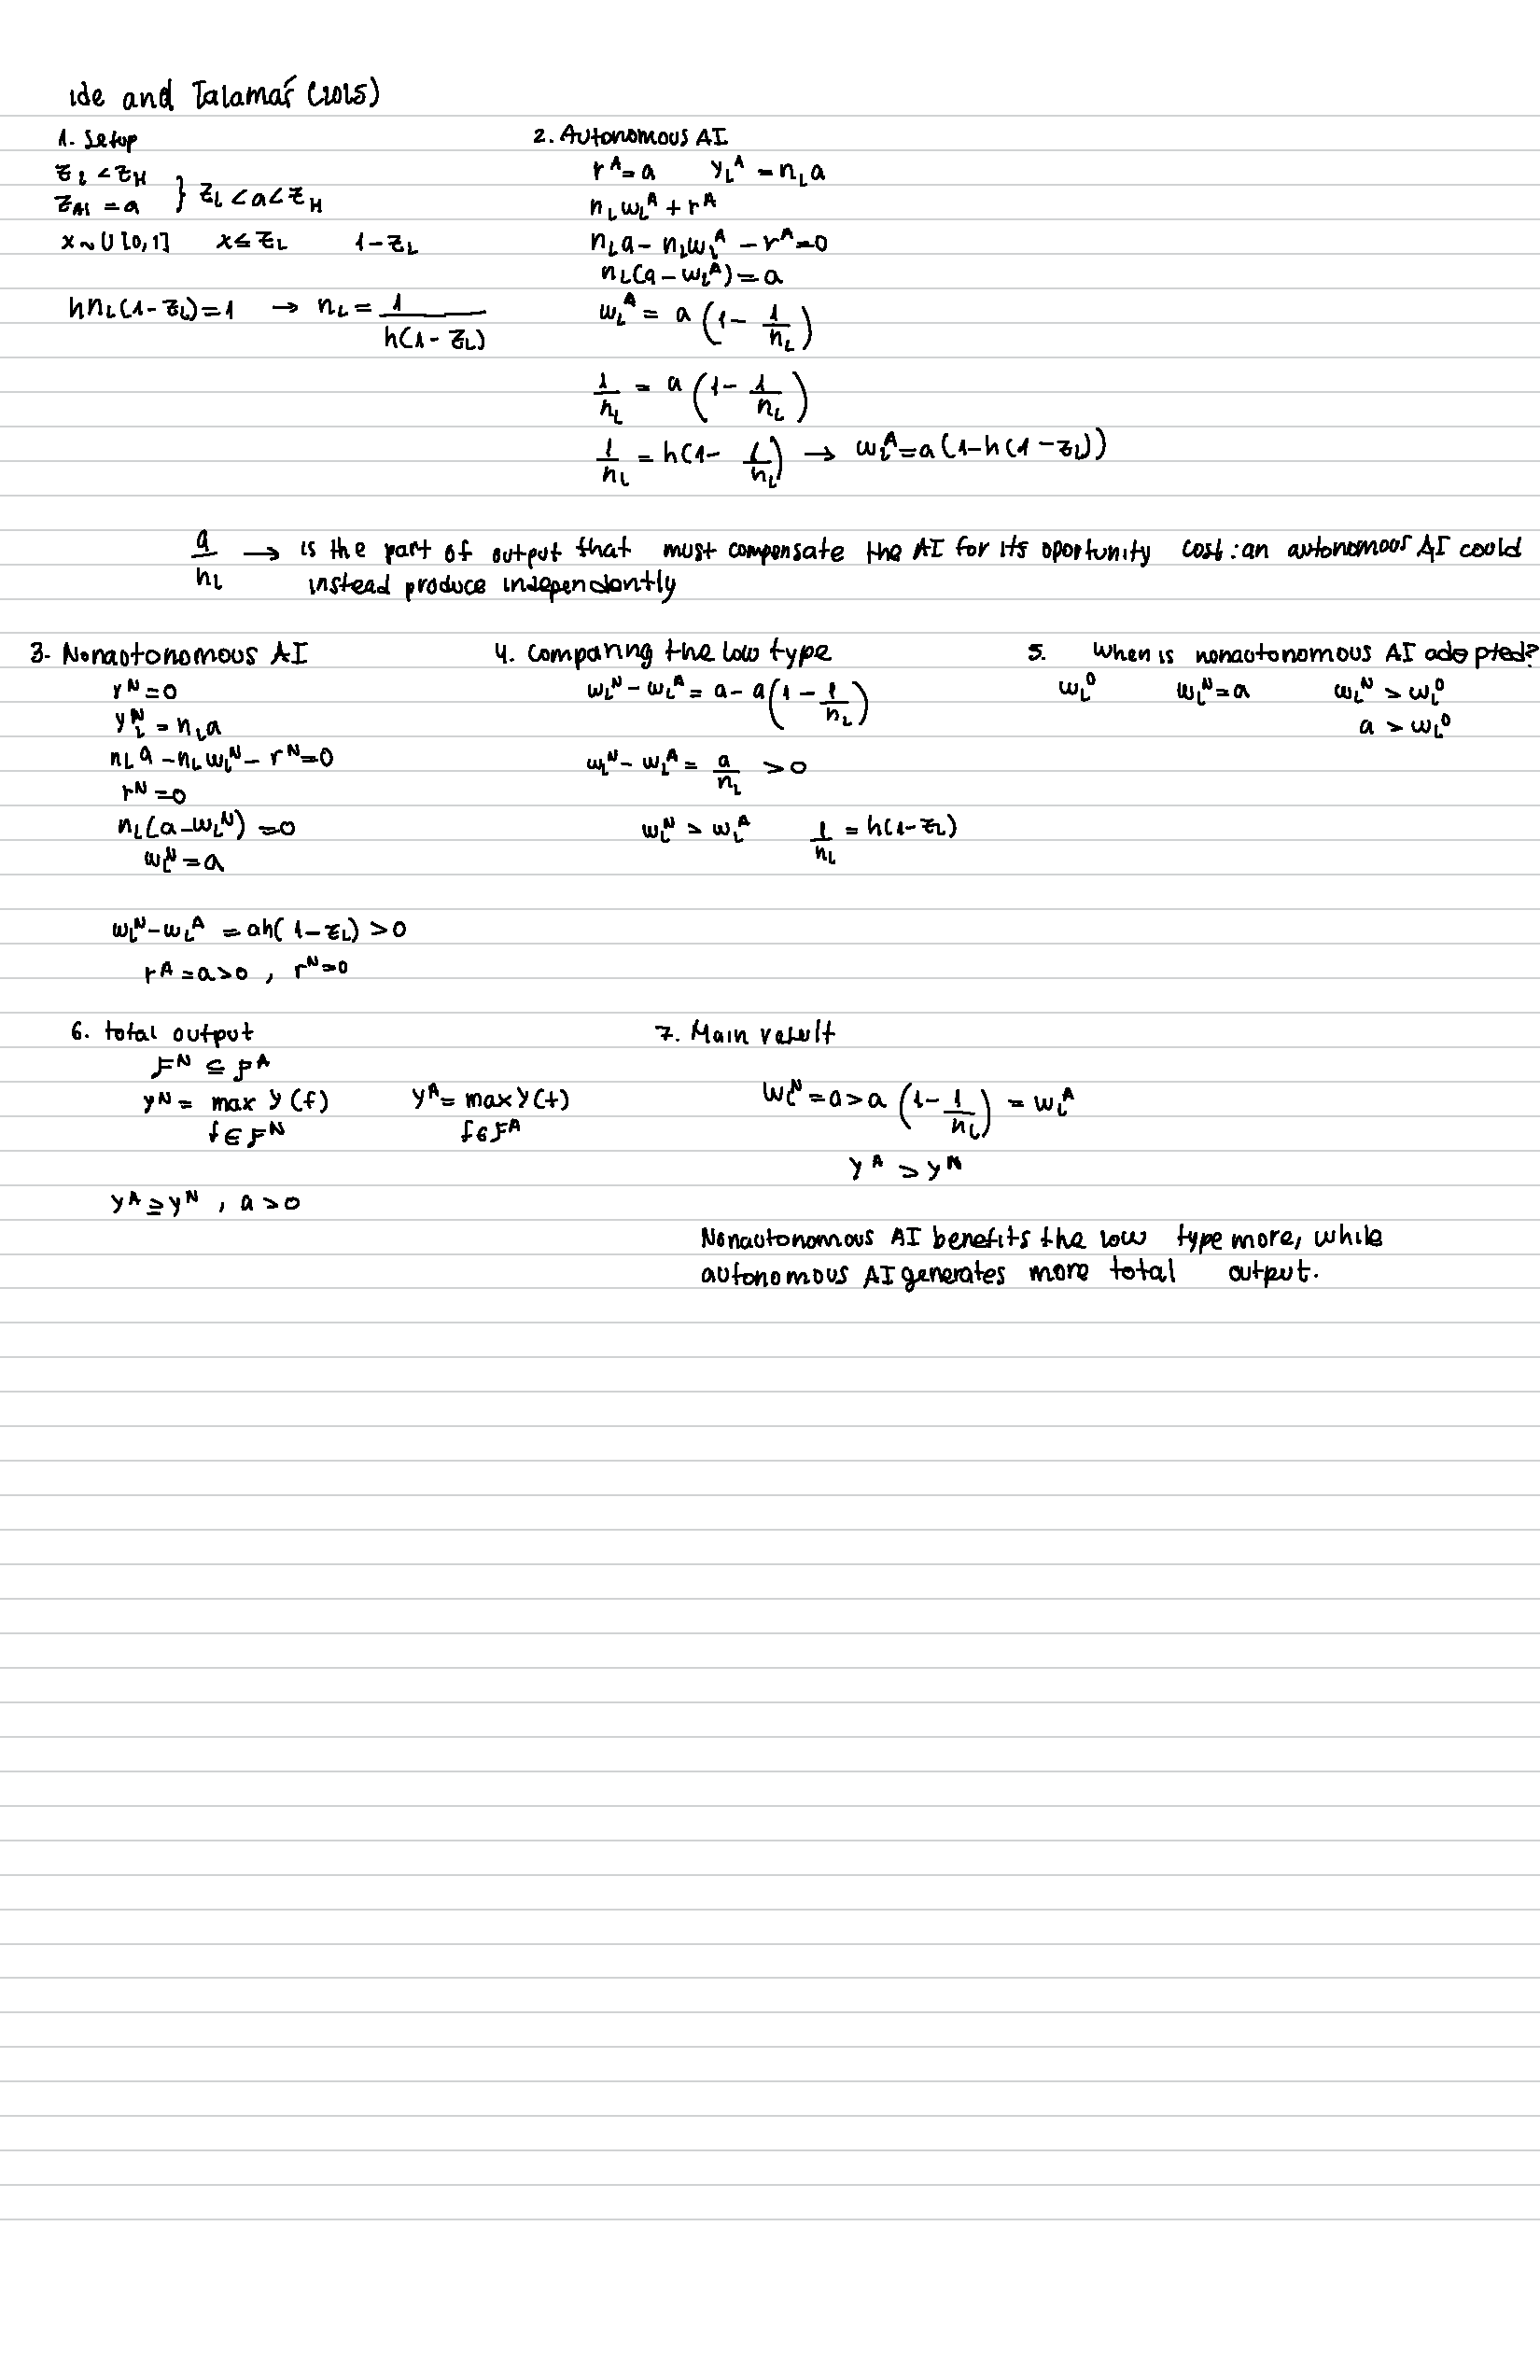
\includegraphics[page=1,width=0.96\linewidth,height=0.67\textheight,trim=20 580 20 22,clip,keepaspectratio]{hand/derivacion_manual_proposicion_6.pdf}}}{\fcolorbox{Turquesa}{white}{\parbox[c][0.60\textheight][c]{0.92\linewidth}{\centering\color{Gris}Inserte aqu\'i la derivaci\'on manual.}}}
{\tiny\color{Gris}Derivaci\'on manual: salarios del tipo bajo y comparaci\'on de producto.}
\end{columns}
\end{frame}

\begin{frame}{Lean: de la ecuaci\'on a la proposici\'on}
\begin{columns}[T,onlytextwidth]
\column{0.48\textwidth}
\clave{Ecuaci\'on matem\'atica}
\[w_L^N-w_L^A=a-a\left(1-\frac1n\right)=\frac an>0,\]
si $a>0$ y $n>1$.
\begin{block}{Frontera de traducci\'on}
Lean verifica la comparaci\'on algebraica discreta. No demuestra que las f\'ormulas salariales emerjan del equilibrio continuo: esas ecuaciones son la interfaz econ\'omica de entrada.
\end{block}
\column{0.48\textwidth}
\clave{Statement Lean}\par
\vspace{0.08cm}
{\fontsize{7.5}{9}\selectfont\ttfamily
def LowTypeWageAdvantageSpec : Prop :=\\
\quad forall \{a n wA wN : Real\},\\
\qquad 0 < a -> 1 < n ->\\
\qquad wA = a * (1 - 1 / n) ->\\
\qquad wN = a -> wN > wA\par}
\vspace{0.25cm}
{\small Las dos igualdades salariales quedan como premisas visibles: Lean audita su consecuencia algebraica, no las ``esconde'' como si ya hubiera formalizado el equilibrio.}
\end{columns}
\end{frame}

\begin{frame}{Lean: qu\'e certifica}
\begin{columns}[T,onlytextwidth]
\column{0.52\textwidth}
\clave{1. Gap salarial del bottom}\par
\vspace{0.08cm}
{\scriptsize\ttfamily
rw [hwA, hwN]\\
have hn0 : 0 < n := lt\_trans zero\_lt\_one hn\\
rw [mul\_sub, mul\_one]\\
exact sub\_lt\_self a\\
\quad (mul\_pos ha (one\_div\_pos.mpr hn0))\par}
\vspace{0.22cm}
{\footnotesize La reescritura deja $a-a(1/n)<a$; Lean certifica que $a(1/n)>0$.}

\vspace{0.23cm}
\clave{2. Puente para producto estricto}\par
{\tiny\ttfamily
0 < extra ->\\
yA = yN + extra -> yA > yN\par}
{\footnotesize Lean exige explicitar \texttt{extra > 0}: la mera inclusi\'on factible solo producir\'ia una desigualdad d\'ebil.}

\column{0.44\textwidth}
\begin{block}{Lectura del certificado}
\begin{itemize}\footnotesize
\item \textbf{S\'i verifica:} que las hip\'otesis escritas bastan y que no hay divisi\'on por cero.
\item \textbf{Detecta:} el supuesto faltante para pasar de $Y^A\ge Y^N$ a $Y^A>Y^N$.
\item \textbf{No verifica:} el equilibrio continuo, los umbrales $\bar z_{AI}$ y $h_0$, ni las Proposiciones 5--6 completas.
\end{itemize}
\end{block}
{\scriptsize\color{Gris}Por eso el repositorio declara el estado como \textit{partially formalized}.}
\end{columns}
\end{frame}

\begin{frame}{Conclusi\'on}
\begin{columns}[T,onlytextwidth]
\column{0.31\textwidth}
\begin{block}{Bottom}
Prefiere relativamente IA no aut\'onoma; con IA aut\'onoma gana solo si la capacidad supera el umbral.
\end{block}
\column{0.31\textwidth}
\begin{block}{Top}
Prefiere IA aut\'onoma bajo $h<h_0$ y $z_{AI}<1$, porque escala su conocimiento sobre m\'as producci\'on.
\end{block}
\column{0.31\textwidth}
\begin{block}{Producto}
La autonom\'ia evita c\'omputo ocioso y eleva el producto: $Y^A>Y^N$.
\end{block}
\end{columns}
\vspace{0.38cm}
\centering
{\Large\color{Noche}\textbf{Autonom\'ia define el conjunto de usos; capacidad define cu\'ando esos usos importan.}}
\vspace{0.28cm}
{\small\color{Petroleo}\repo}
\end{frame}

\end{document}
